\chapter{The results, and what each one really says}
\label{ch:results}

\section{The main table}
\begin{center}
\scriptsize
\setlength{\tabcolsep}{3pt}
\begin{tabular}{lcccccc}
\toprule
Engine & Detected [95\% CI] & A@1 & A@3 & C+N [95\% CI] & FA/h & Alarm \%\\
\midrule
\multicolumn{7}{l}{\textit{Real benches (62 faults, 217 min)}}\\
Rules & 90 [82, 97] & 70 & 91 & 63 [52, 74] & 9.2 & 9\\
Severity ranking & 90 [82, 97] & 75 & 86 & 68 [56, 79] & 6.2 & 8\\
ML engine & 90 [82, 97] & 79 & 89 & 71 [60, 81] & 2.3 & 6\\
\textbf{Hybrid} & 90 [82, 97] & 79 & 89 & 71 [60, 81] & 6.2 & 8\\
Hybrid + change-point & 95 [89, 100] & 76 & 88 & 73 [61, 82] & 5.4 & 16\\
Hybrid + learned dir. & 90 [82, 97] & 75 & 89 & 68 [55, 77] & 6.2 & 8\\
\midrule
\multicolumn{7}{l}{\textit{Synthetic held-out (178 faults, 16 topologies)}}\\
Rules & 89 [84, 93] & 78 & 95 & 70 [62, 76] & 2.5 & 2\\
Severity ranking & 93 [89, 97] & 80 & 92 & 74 [67, 80] & 0.9 & 5\\
ML engine & 92 [87, 96] & 82 & 94 & 75 [69, 81] & 0.2 & 4\\
\textbf{Hybrid} & 93 [89, 97] & 81 & 93 & 75 [69, 81] & 0.9 & 5\\
Hybrid + change-point & 94 [90, 98] & 80 & 92 & 75 [69, 81] & 0.8 & 6\\
Hybrid + learned dir. & 93 [89, 97] & 81 & 93 & 75 [69, 81] & 0.9 & 5\\
\bottomrule
\end{tabular}
\end{center}

\begin{simplebox}
How to read it, row by row for the real benches. \textbf{Rules} found 90\% of faults, and named the right service first for 63\% of all faults, but they raised 9.2 false alarms per hour and were in alarm 9\% of the fault-free time. \textbf{ML} found the same 90\%, named the right service for 71\%, and raised only 2.3 false alarms per hour (6\% alarm time). \textbf{Hybrid} (the default) has the same 71\% but 6.2 false alarms per hour, because it also lets the rules raise the alarm. The two bold results to stress: ML and Hybrid have higher C+N than Rules, and ML has by far the fewest false alarms.
\end{simplebox}

\begin{techbox}
Paired differences (C+N): Hybrid vs Rules $+8.1$ points on the real systems (95\% CI $[-1.6,+17.7]$, $p=0.117$), $+5.6$ on the synthetic set ($[-0.6,+11.8]$, $p=0.093$); Hybrid vs severity ranking $+3.2$ and $+1.1$; Hybrid vs ML $0.0$ and $+0.6$. The first version of the report showed hybrid over rules as significant ($+9.7$ points, $p=0.032$). With the corrected engine it is not: the improvement is in robustness, not in the benchmark. With 62 real faults a difference below about ten points cannot be resolved.
\end{techbox}

\begin{figure}[H]
\centering
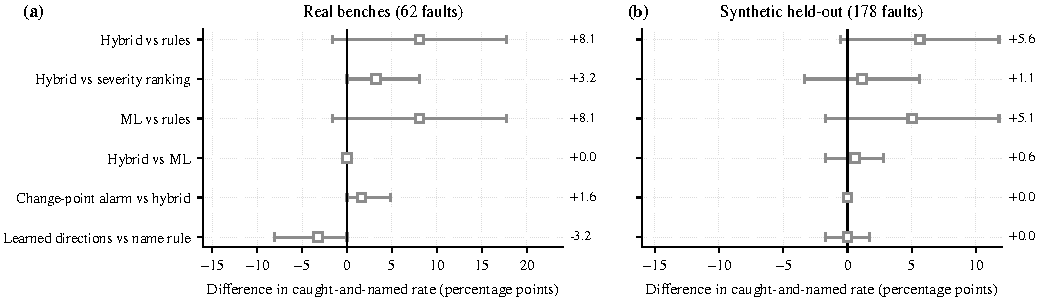
\includegraphics[width=0.98\textwidth]{fig_forest.pdf}
\caption{Paired differences in caught-and-named rate between engines (percentage points, 95\% paired-bootstrap interval); filled markers exclude zero.}
\end{figure}

\begin{figure}[H]
\centering
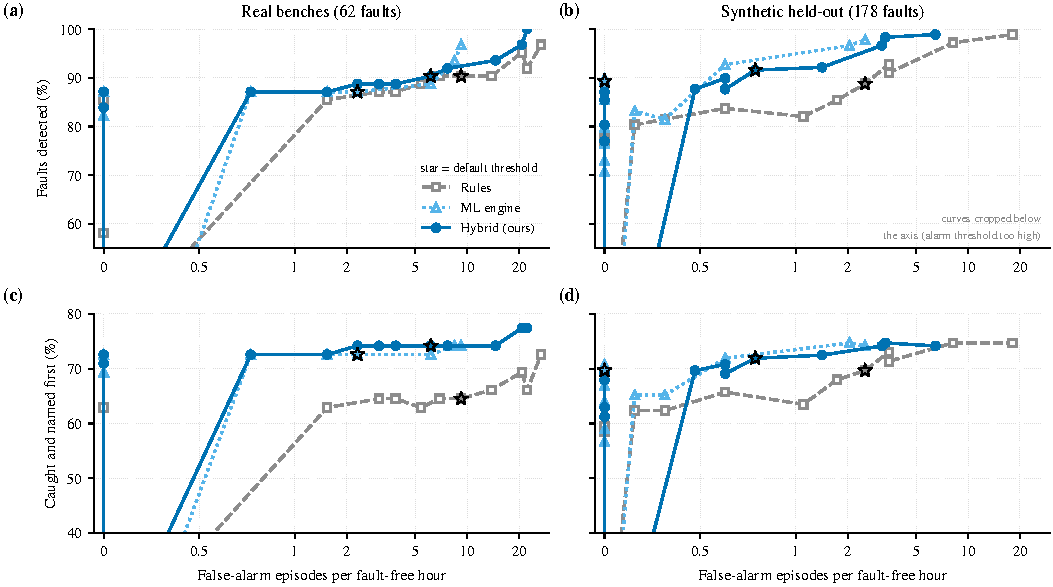
\includegraphics[width=0.98\textwidth]{fig_op.pdf}
\caption{Operating curves. Sweeping the alarm threshold of each engine traces detection rate (top) and caught-and-named rate (bottom) against false-alarm episodes per hour; stars mark the default threshold.}
\end{figure}

\begin{simplebox}
The operating curves show a different way to compare engines. Every engine has a dial (the alarm threshold). Turning the dial up trades faults caught for fewer false alarms. If you plot that trade for every engine, you see whether one engine is better at \emph{every} dial setting. Here the curves are close, and Hybrid and ML sit on or near the top edge in both sets, above the rules at almost every false-alarm budget. So their advantage is about the \emph{operating point}, not one lucky threshold.
\end{simplebox}

\begin{saybox}
``Rules, ML and Hybrid are close on how many faults they catch, 90\% on the real systems. The difference is that ML and Hybrid name the right service more often, 71\% against 63\%, and ML does it with a quarter of the false alarms. The 71 against 63 is not statistically significant with 62 faults, and we say so.''
\end{saybox}

\section{The ablation: which part matters}
\begin{figure}[H]
\centering
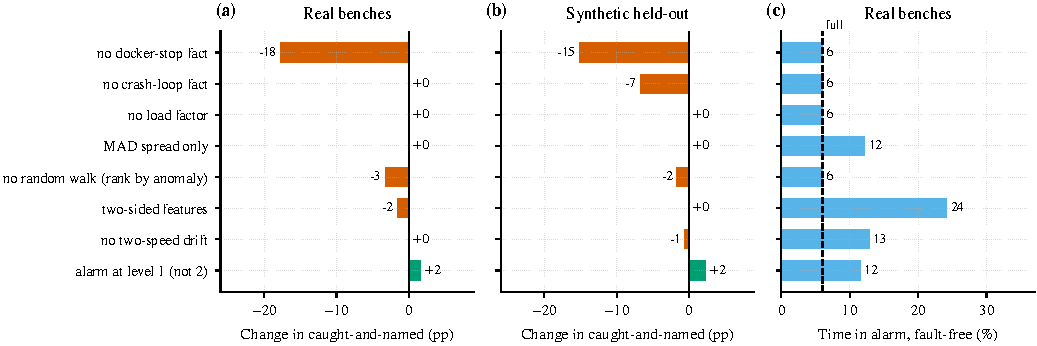
\includegraphics[width=0.98\textwidth]{fig_ablation.pdf}
\caption{Ablation. Each bar removes one mechanism from the full engine.}
\end{figure}

\begin{simplebox}
An ablation takes the full tool and removes one part at a time, to see what that part was worth. The parts are, in order of importance:
\begin{enumerate}
\item \textbf{The \code{docker stop} fact} costs \textbf{18 points} on the real systems and 15 on the synthetic set when removed, because every stopped service goes unnamed. This is the single most valuable component.
\item \textbf{The crash-loop fact}: 0 points on the real systems and 7 on the synthetic set.
\item \textbf{The random walk}: 3 and 2 points.
\item \textbf{The load factor}: nothing changes on injected faults (the load does not move in them); it matters on the workload recordings, where false alarms go from 0.0 to 1.2 and from 1.0 to 1.9 per hour without it.
\item \textbf{The tail-aware spread}: with the plain MAD spread, alarm time on the real systems doubles (6\% to 12\%), and on the workload recordings rises from 0\% to 10\% and 6\%.
\item \textbf{One-sided features}: removing them raises alarm time on the real systems from 6\% to 24\%.
\item \textbf{The two-speed drift}: without it, alarm time is 13\% instead of 6\% and false alarms 3.1 instead of 2.3 per hour.
\end{enumerate}
\end{simplebox}

\begin{saybox}
``The most important single component is container state as a fact: 18 points. The statistical mechanisms matter in a different way: they decide whether the model stays \emph{quiet}, not whether it \emph{catches} faults. Without the load factor nothing changes on the injected faults, but with it the false alarms on the workload recordings go from 1.2 and 1.9 per hour to 0.0 and 1.0.''
\end{saybox}

\section{Detection delay and top-$k$}
\begin{simplebox}
How fast does it react? On the real systems, the Hybrid's median delay from the start of a fault to the first alarm is 11.3 seconds, against 14.9 for the rules. On the synthetic set, whose faults are abrupt, it is 8.2 against 9.5 seconds. And among the detected faults, ML-based rankers put the true cause first more often than rules on the real systems (79\% against 70\%); by the third place both are near the 90\% ceiling. The remaining misses are mostly faults the engine \emph{does not see} (brownouts on near-idle services), not faults it ranks badly.
\end{simplebox}

\section{The service-level detection table}
\begin{center}
\small
\begin{tabular}{lcccc}
\toprule
 & \multicolumn{2}{c}{Real} & \multicolumn{2}{c}{Synthetic}\\
Detector & AUROC & AP & AUROC & AP\\
\midrule
Rule z-score & 0.695 & 0.337 & 0.873 & 0.666\\
Isolation Forest (old) & 0.629 & 0.288 & 0.862 & 0.528\\
k-NN & 0.668 & 0.193 & 0.860 & 0.517\\
Mahalanobis & 0.650 & 0.290 & 0.868 & 0.608\\
HBOS & 0.620 & 0.274 & 0.853 & 0.473\\
Ensemble of four & 0.650 & 0.287 & 0.865 & 0.593\\
Control chart (no load factor) & 0.669 & 0.302 & 0.842 & 0.657\\
Subspace residual & 0.696 & 0.298 & 0.847 & 0.629\\
Load-aware residual (new) & 0.665 & 0.313 & 0.842 & 0.665\\
\bottomrule
\end{tabular}
\end{center}
\begin{simplebox}
\textbf{AUROC} asks: if I pick one faulted service-moment and one healthy one at random, how often does the detector give the faulted one a higher score? 1.0 is perfect, 0.5 is coin-flip. \textbf{AP} (average precision) summarises how pure the top of the ranking is. The plain rule score is among the best on AUROC. That is fine: it ranks single readings well. It is not enough because it also fires on traffic swings and blames the loudest service.
\end{simplebox}

\section{The live campaigns and the auto-restart question}
\begin{center}
\small
\begin{tabular}{llrrrrr}
\toprule
Bench & Auto-restart & Detected & Top-1 (\%) & Top-3 (\%) & Delay (s) & FA/h\\
\midrule
ShopFlow & on & 100\% & 33 [17, 55] & 71 [50, 86] & 3.3 & 9.2\\
ShopFlow & off & 100\% & 24 [11, 45] & 71 [50, 86] & 2.6 & 0.0\\
LedgerLine & on & 95\% & 55 [34, 74] & 65 [43, 82] & 9.7 & 0.0\\
LedgerLine & off & 95\% & 40 [22, 61] & 70 [48, 85] & 3.9 & 3.1\\
\bottomrule
\end{tabular}
\end{center}
\begin{simplebox}
The same plan of 21 faults was replayed four times: both benches, with auto-restart on and off. Almost every fault was detected (all but one), and the true cause was within the top three suspects for 65 to 71\% of faults. The on/off rows differ by 9 to 15 points of Top-1, but with only 21 faults their intervals overlap completely, so none of the differences can be called an effect of auto-restart. \emph{Why was there no effect?} Because the benches set \code{restart: always} (Docker revives a crashed container within seconds, before the mapper looks), the mapper checks for dead containers only every 180 seconds (longer than the 20-second crash faults), and it skips containers that exited with code 0, which is what \code{docker stop} produces. The one restart in each ``on'' run was of the \emph{other} bench's message bus, which we had stopped by hand; that is an artefact of the setup and the report says so.
\end{simplebox}

\begin{techbox}
Direct test: \code{cart} and \code{payments} were each stopped for 5 minutes by the Fault Lab, sampled every 2\,s. Down time with auto-restart on/off: cart 299\,s / 298\,s, payments 301\,s / 301\,s. The mapper left the containers down in both modes. Brownouts are the weak class in all four runs (no Top-1 at all).
\end{techbox}

\section{The engines on one live fault (the simulator story)}
\begin{simplebox}
We also ran a simulator with a slow \code{payment} service (CPU saturated from second 30; \code{orders} follows twelve seconds later). It shows the personality of each engine on one fault.

\begin{center}
\small
\begin{tabularx}{\textwidth}{>{\raggedright\arraybackslash}p{1.6cm}>{\raggedright\arraybackslash}X>{\raggedright\arraybackslash}X>{\raggedright\arraybackslash}X}
\toprule
Engine & +5 s: payment only & +20 to +70 s: both saturated & after +75 s\\
\midrule
Rules & payment (3.0$\times$) & orders (3.7$\times$), payment second & the same\\
ML & payment (88\% of the walk) & payment (57\%), orders (43\%) & absorbed: no alarm\\
Hybrid & payment & payment (0.91), orders (0.87) & orders (alarm kept by the rules)\\
\bottomrule
\end{tabularx}
\end{center}

Rules point at the \emph{loudest} service (orders) once both are saturated. ML keeps blaming \code{payment} because its own CPU is the root, but then, because the fault is steady and mild, absorbs it after two minutes of simulated readings. Hybrid keeps the alarm up (from the rules) while naming the source mostly by ML.
\end{simplebox}

\begin{warnbox}
This is one simulated fault, an illustration and not evidence. It shows the mechanism the evaluation measures at scale. Do not use it as a result.
\end{warnbox}

\section{Operational findings from the benchmark hosts}
\begin{itemize}
\item \textbf{A host too small for its workload looks like a mapper fault.} The OpenTelemetry demo on a 2-vCPU, 4\,GiB instance had a load average near 25, 3.6 of 3.8\,GiB memory in use, and docker did not answer. The check tool measured it; the cure was a bigger host, not a mapper change.
\item \textbf{Idle front ends have no edges.} A front end that nothing calls has no outgoing sockets to see; an undeclared edge expires ten minutes after its last traffic.
\item \textbf{Hard-coded project names blocked traffic.} The traffic controller accepted only five named projects, so benchmark hosts with other names could not be driven. Unknown projects now get a generic workflow.
\end{itemize}

\section{Where we compare with published methods}
\begin{simplebox}
We did \emph{not} re-implement published root-cause systems (MicroRank, DiagFusion, Eadro and others) on our recordings. They need tracing in every service, or labelled failures and a GPU, which our setting does not have. So there is no head-to-head accuracy table against them, and we say that plainly. What we compared head-to-head are the \emph{baselines those methods build on}: the rule layer, ranking by anomaly alone, the walk, and a range of detectors.
\end{simplebox}
